\newpage
\section{Auswertung}
\label{sec:Auswertung}
In diesem Abschnitt werden die aufgenommenen Messdaten in Grafiken dargestellt und ausgewertet. Grafiken sowie dazugehörige Rechnungen sind mit Python \cite{python} erstellt bzw. berechnet worden.
\subsection{Justierung}
Im ersten Auswertungsabschnitt des Versuches, werden zunächst zur Justage von Apparatur und Probe einige Scans aufgenommen und später benötigte Parameter erfasst.
\subsubsection{Detektorscan}
Wie in Abschnitt (\ref{sec:Durchführung}) beschrieben, wird zu Beginn ein Detektorscan durchgeführt. Die aufgenommenen Daten sind Abbildung (\ref{fig:detekscan}) zu finden.
\begin{figure}[h!]
  \centering
  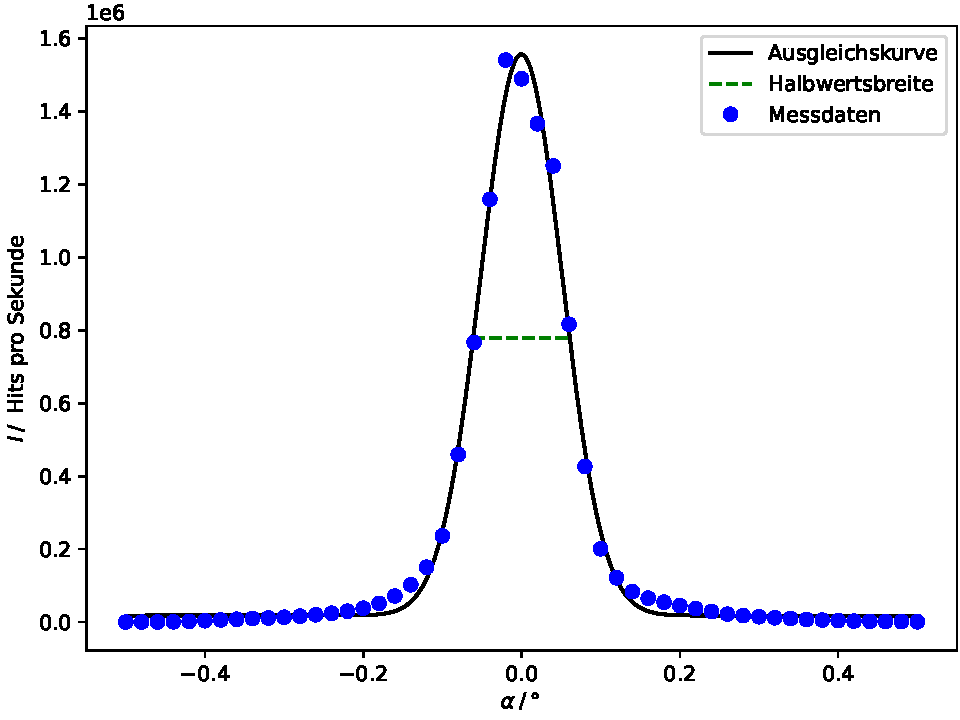
\includegraphics[scale=0.7]{fig/plot_detektorscan.pdf}
  \caption{Messdaten des Detektorscan mit Gaußfunktion.}
  \label{fig:detekscan}
\end{figure}
Die Ausgleichsfunktion hat die Form einer Gaußfunktion und ist gegeben durch:
\begin{equation}
  \label{eqn:detektor}
  I(\alpha)=\dfrac{a}{\sqrt{2\pi\sigma^2}}\exp\left(-\dfrac{(x-\mu)^2}{2\sigma^2}\right)+b
\end{equation}
Die Parameter ergeben sich zu:
\begin{align*}
  a &= \SI{1.98(3) e5}{} \\
  b &= \SI{1.8(5) e4}{} \\
  \sigma &= \SI{0.0513(8)}{\degree} \\
  \mu &= \SI{0.002(7)}{\degree}
\end{align*}
Jetzt werden noch die maximale Intensität $I_\mathrm{max}$ und die Halbwertsbreite von der Gaußfunktion abgelesen. Diese lauten:
\begin{align*}
  \mathrm{HWB}&=0.122 \\
  I_\mathrm{max}&=\SI{1.557 e6}{}
\end{align*}
\subsubsection{Z-Scan}
In diesem Abschnitt wird aus dem aufgenommen Z-Scan die Strahlbreite $d_\mathrm{0}$ bestimmt. Die Strahlbreite ist der Abstand zwischen minimaler und maximaler Intesität. In Abbildung (\ref{fig:zscan}) ist dies grafisch dargestellt:
\begin{figure}[h!]
  \centering
  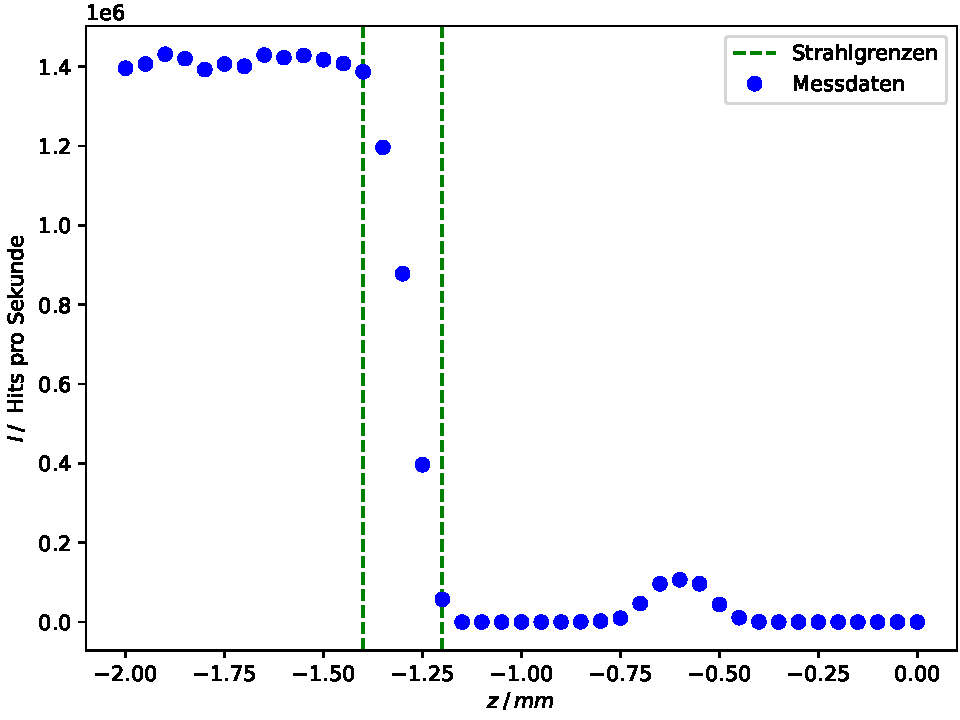
\includegraphics[scale=0.7]{fig/plot_zscan.pdf}
  \caption{Messdaten des Z-Scan mit Strahlbreite $d_\mathrm{0}$.}
  \label{fig:zscan}
\end{figure}
\FloatBarrier
\noindent Damit ergibt sich die Strahlbreite zu:
\begin{equation*}
  d_\mathrm{0}=\SI{0.2}{\milli\meter}
\end{equation*}
\subsubsection{Rockingscan}
Im letzten Teil der Justage wird aus dem aufgenommenen Rockingscan der Geometriewinkel $\alpha_\mathrm{g}$ bestimmt.
Dazu ist in Abbildung (\ref{fig:rockscan}) das Ergebnis des Scans grafisch dargestellt:
\begin{figure}[h!]
  \centering
  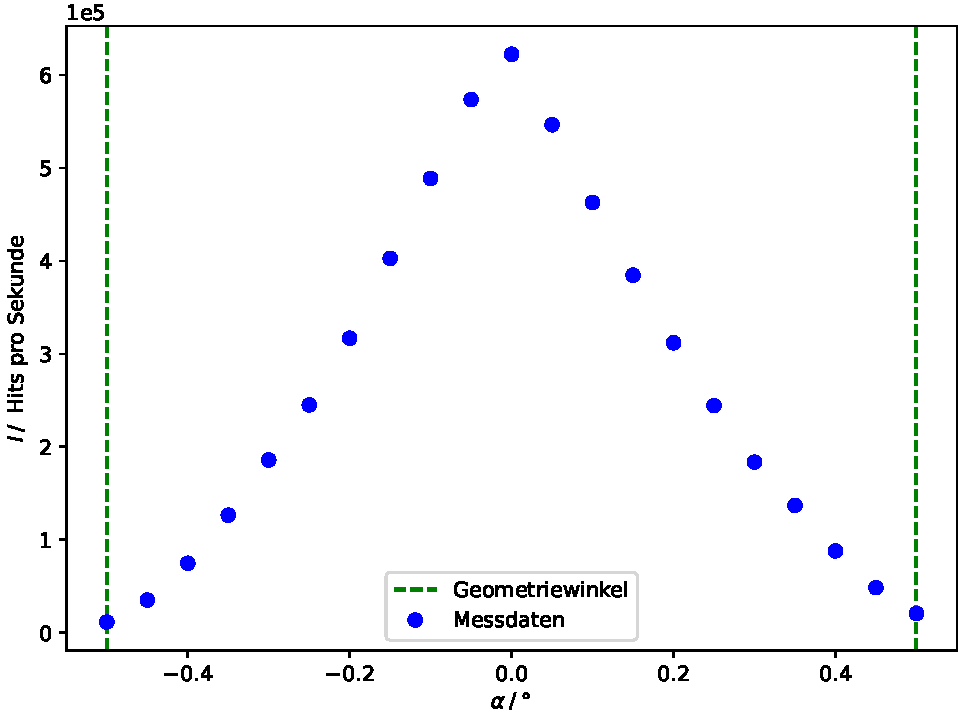
\includegraphics[scale=0.7]{fig/plot_rockingscan.pdf}
  \caption{Messdaten des Rockingscan mit Geometriewinkeln $\alpha_\mathrm{0}$.}
  \label{fig:rockscan}
\end{figure}
\FloatBarrier
\noindent Die beiden abgelesenen Geometriewinkel sowie der gemittelte Wert lauten:
\begin{align*}
  \alpha_\mathrm{g,links} &= \SI{0.5}{\degree} \\
  \alpha_\mathrm{g,rechts} &= \SI{0.5}{\degree} \\
  \overline{\alpha}_\mathrm{g} &= \SI{0.5}{\degree}
\end{align*}
Mit Gleichung (\ref{eqn:Geometriewinkel}) kann mit der ermittelten Strahlbreite $d_\mathrm{0}=\SI{0.2}{\milli\meter}$ sowie der Probenlänge $D=\SI{20}{\milli\meter}$ ein theoretischer Wert
für den Geometriewinkel bestimmt werden. Dieser ergibt sich zu:
\begin{equation*}
  \alpha_\mathrm{g,Theorie} = \SI{0.573}{\degree}
\end{equation*}
\subsection{Bestimmung des Dipersionsprofil}
In diesem Abschnitt wird aus dem aufgenommenen Reflektivitätsscan das Dipersionsprofil der Probe bestimmt. In Abbildung (\ref{fig:messungr}) sind die Ergebnisse zusammengefasst:
\begin{figure}[h!]
  \centering
  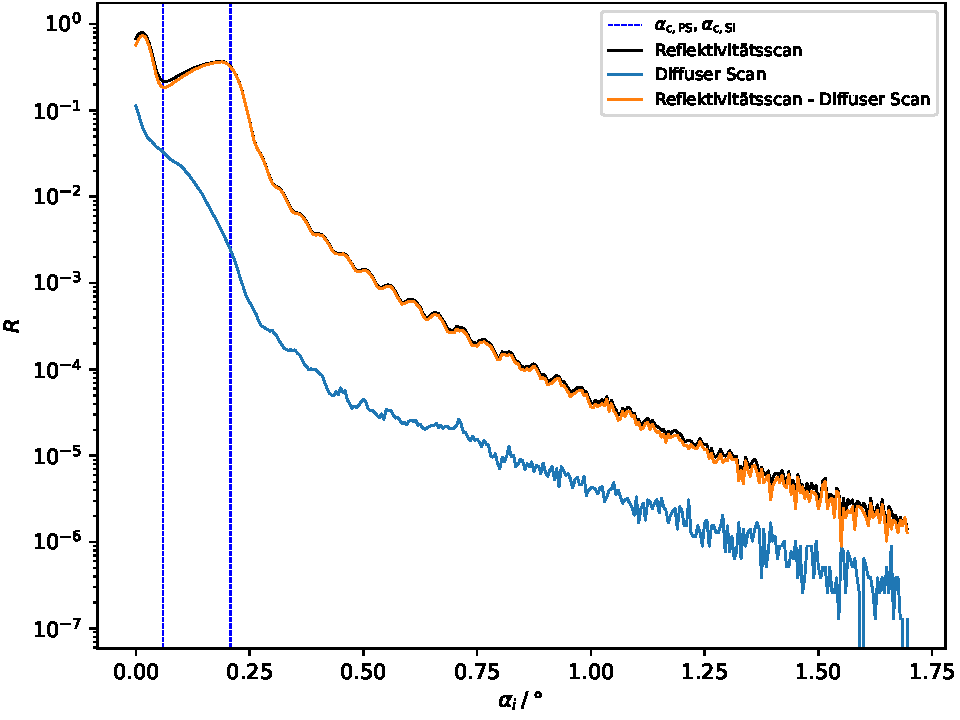
\includegraphics[scale=0.7]{fig/plot_messung.pdf}
  \caption{Grafische Zusammenfassung der gewonnenen Messdaten.}
  \label{fig:messungr}
\end{figure}
\FloatBarrier
\noindent Da die Messdaten im Bereich $\alpha_\mathrm{e} > \SI{1.7}{\degree}$ nicht aussagekräftig sind, werden diese in der Grafik nicht angezeigt. Die Reflektivität $R$ ergibt sich mit einer Abtastrate von 5 aus folgender Formel:
\begin{equation}
  R=\dfrac{I}{5\cdot I_\mathrm{max}}
\end{equation}
Der aufgenommene diffuse Scan wird, um Streueffekte so gut wie möglich zu unterdrücken, vom Reflektivitätsscan abgezogen. Da die gemessenen Intesitäten beim diffusen Scan gering waren, fällt
dies in der Grafik kaum auf. Die Reflektivität wird mit einem Geometriefaktor korrigiert, dieser ergibt sich mit den aus der Justage ermittelten Größen nach Gleichung (\ref{eqn:Geometriefaktorl}). Außerdem ist in Abbildung (\ref{fig:messungr}) zu Vergleichszwecken die Fresenelreflektivität einer ideal glatten Siliziumoberfläche  aufgetragen.
Diese wird aus dem Literaturwert \cite[5]{Anleitung3} $\alpha_\mathrm{c,Silizium} = \SI{0.223}{\degree}$ mit Hilfe von Gleichung (\ref{eqn:Fresnelref}) bestimmt. \\
\\
\subsubsection{Reflektivitätsmessung}
Zur Bestimmung der Schichtdicke der Polystyrolschicht werden aus dem durch den Geometriefaktor korrigierten Reflektivitätsscan die Abstände $\Delta\alpha_\mathrm{e}$ der Minima der Kiessig-Oszillation
ermittelt. Der Mittelwert dieser Abstände ergibt sich zu:
\begin{equation}
  \overline{\Delta\alpha}_\mathrm{e} = \SI{8.8(3) e-4}{\degree}
\end{equation}
Die Schichtdicke berechnet sich aus Gleichung (\ref{eqn:Schichtdicke}) mit $\lambda=\SI{1.54 e-10}{\meter}$ zu:
\begin{equation*}
  d_\mathrm{PS}=\SI{8.7(3) e-8}{\meter}
\end{equation*}
\subsubsection{Parratt-Algorithmus}
In diesem Abschnitt wird ebenfalls die Schicktdicke sowie die kritischen Winkel der verschiedenen Substanzen ermittelt. Dazu wird der Parratt-Algorithmus aus Abschnitt (\ref{sec:Mehrschichtensysteme}) verwendet.
Als erstes wird dafür die Reflektivität $R$ für den jeweiligen Einfallswinkel $\alpha_\mathrm{e}$ aus den Gleichungen (\ref{eqn:Parratt-Algorithmus}), (\ref{eqn:kzj}) und (\ref{eqn:modkoeff}) berechnet.
Die hier betrachteten Schichten sind Luft (Schicht 1), Polystyrol (Schicht 2) und Silizium bzw. Substrat (Schicht 3). Da das Substrat als unendlich dick angenommen wird und damit die transmittierte Strahlung $t_\mathrm{N+1}$ nicht mehr reflektiert wird ergibt sich für $r_\mathrm{N+1}=0$, der als Startwert dient. Die bekannten Parameter sind gegeben durch:
\begin{align*}
  \delta_\mathrm{1,Luft}&=0 \\
  z_\mathrm{1}&=0 \\
  \lambda&=\SI{1.54 e-10}{\meter}
\end{align*}
Die weiteren Parameter $\delta_\mathrm{2}$, $\delta_\mathrm{3}$, $\sigma_\mathrm{1}$, $\sigma_\mathrm{2}$ und $z_\mathrm{2}$ werden so gewählt, dass die Theoriekurve und die gemessene Reflektivität so gut wie möglich übereinstimmen.
Die Theoriekurve aus Abbildung (\ref{fig:messungr}) hat die folgenden Parameter:
\begin{align*}
  \delta_\mathrm{2,PS} &=\SI{0.55 e-6}{} \\
  \delta_\mathrm{3,Si} &=\SI{6.6 e-6}{} \\
  \sigma_\mathrm{1} &=\SI{7.5 e-10}{\meter} \\
  \sigma_\mathrm{2} &=\SI{6.3 e-10}{\meter} \\
  z_\mathrm{2} &=\SI{8.6 e-8}{\meter}
\end{align*}
Aus den  Dispersionen für Polystyrol $\delta_\mathrm{PS}$ und Silizium $\delta_\mathrm{Si}$ werden die kritischen Winkel $\alpha_\mathrm{c}$ bestimmt. Dafür wird Gleichung (\ref{eqn:Totalreflexion}) verwendet und die folgenden Werte ergeben sich:
\begin{align*}
  \alpha_\mathrm{c,PS} &=\SI{0.06}{\degree} \\
  \alpha_\mathrm{c,Si} &=\SI{0.208}{\degree}
\end{align*}
Diese sind in Abbildung (\ref{fig:messungr}) durch die gestrichelten Linien gekennzeichnet.
%\begin{figure}[h!]
%  \centering
%  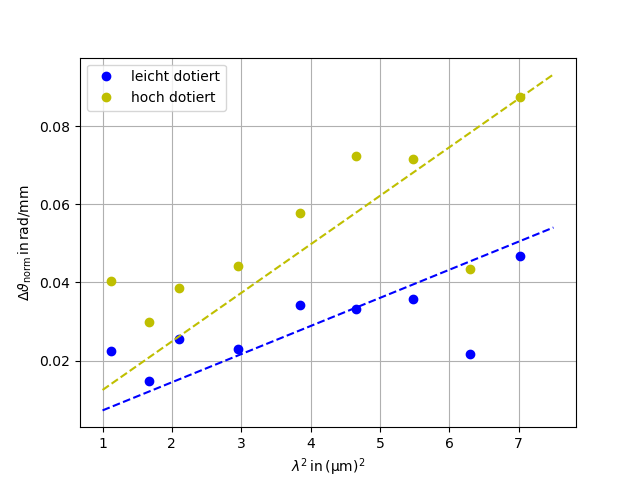
\includegraphics[scale=0.7]{fig/deltaTheta.png}
%  \caption{Grafische Darstellung der Messdaten aus den Tabellen \ref{tab:tief} und \ref{tab:hoch}.}
%  \label{abb:delta}
%\end{figure}
